\documentclass{standalone}
\usepackage{tikz}
\usetikzlibrary{shapes.geometric}
\usetikzlibrary{patterns, positioning}


\begin{document}
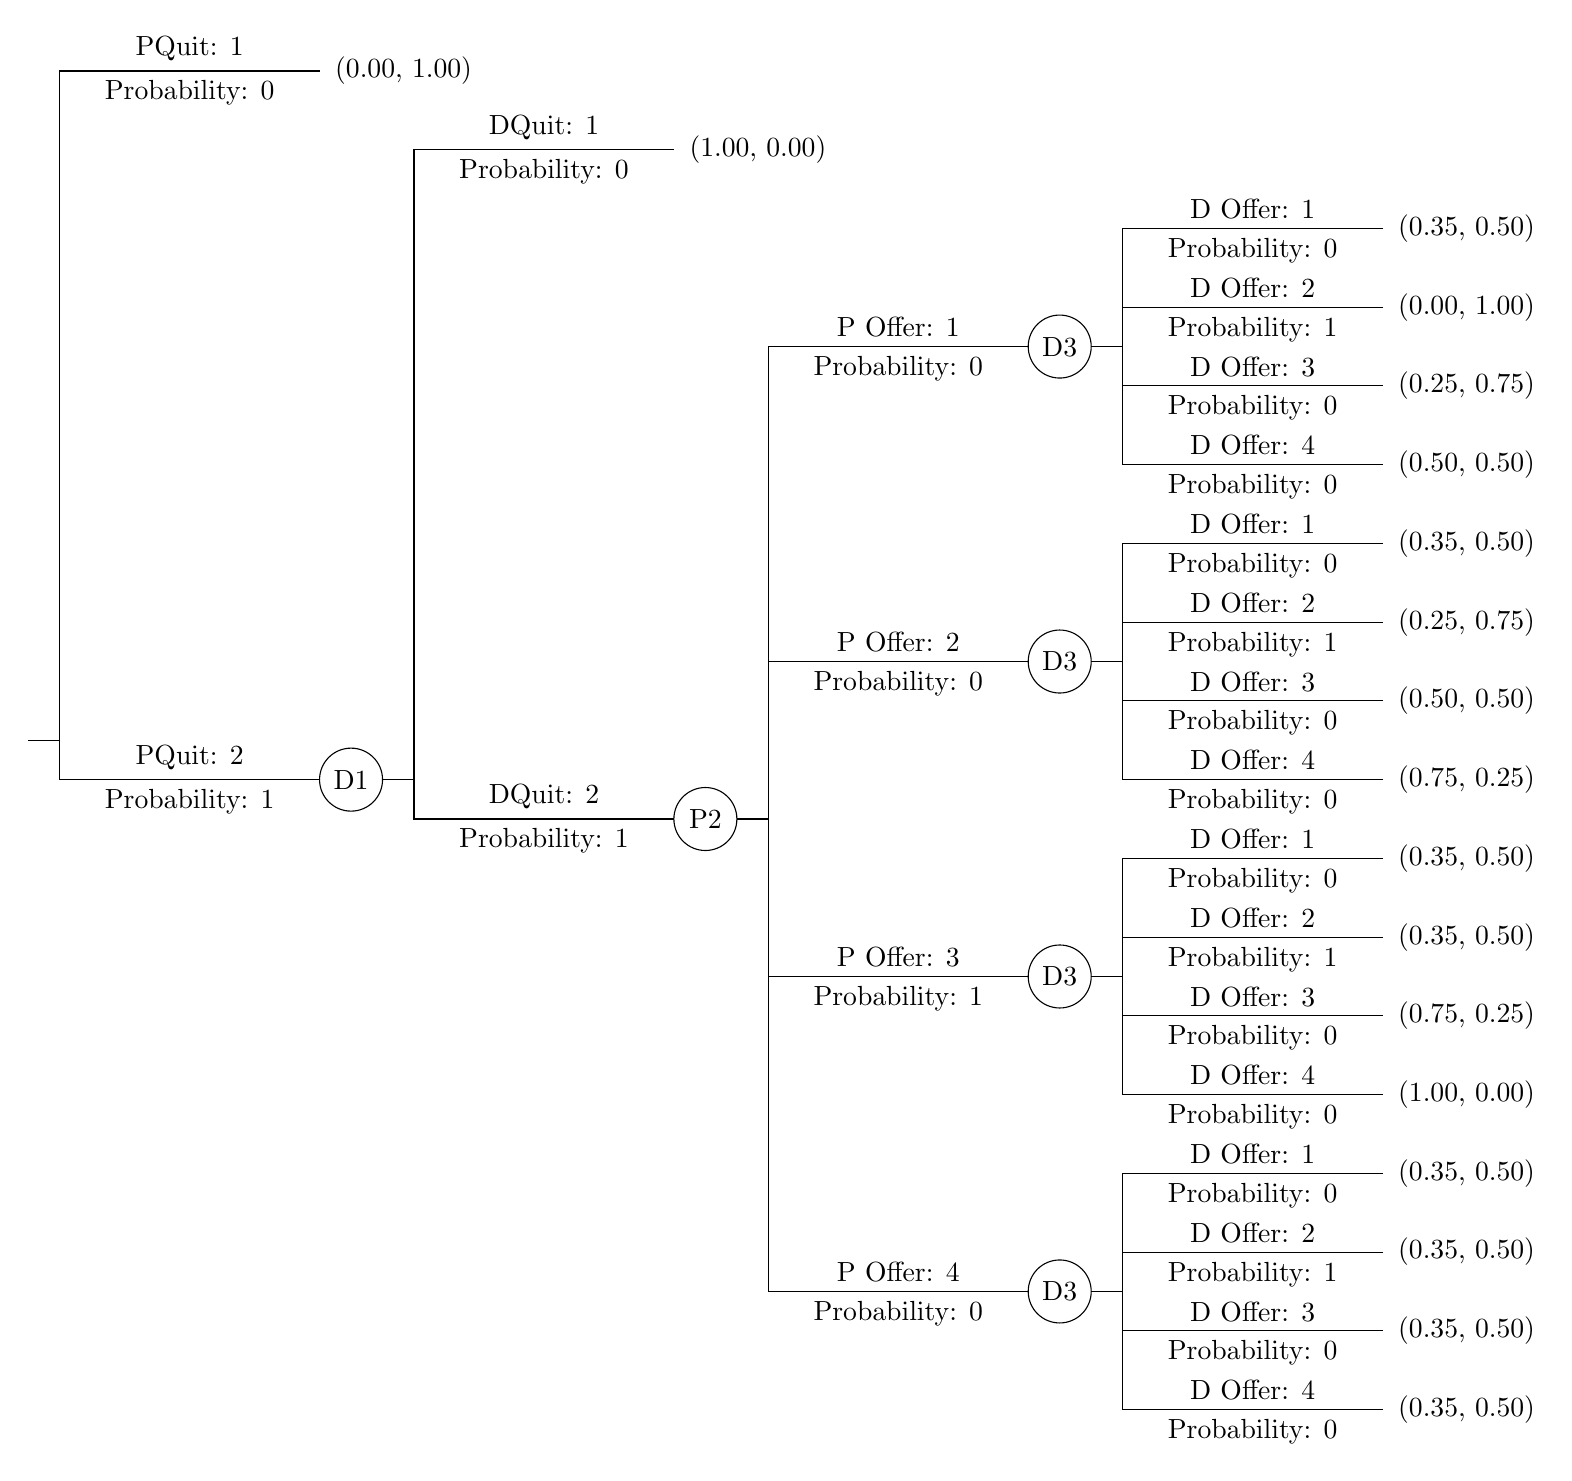
\begin{tikzpicture}

    \draw[color=black] (-13.5, -0.25) node[draw=none] (N0) {};
\node[draw=none, right=-0.45cm of N0] {(0.00, 1.00)};
\draw (-17.6, -8.75) -- (-17.200000000000003, -8.75) -- (-17.200000000000003, -0.25) -- (-13.9, -0.25) node [midway, above, sloped] (E0) {PQuit: 1} node [midway, below, sloped] (E1) {Probability: 0} ;


    \draw[color=black] (-13.5, -9.25) circle (0.4cm) node[draw=none] (N2) {D1};
\draw (-17.6, -8.75) -- (-17.200000000000003, -8.75) -- (-17.200000000000003, -9.25) -- (-13.9, -9.25) node [midway, above, sloped] (E2) {PQuit: 2} node [midway, below, sloped] (E3) {Probability: 1} ;


    \draw[color=black] (-9, -1.25) node[draw=none] (N4) {};
\node[draw=none, right=-0.45cm of N4] {(1.00, 0.00)};
\draw (-13.1, -9.25) -- (-12.7, -9.25) -- (-12.7, -1.25) -- (-9.4, -1.25) node [midway, above, sloped] (E4) {DQuit: 1} node [midway, below, sloped] (E5) {Probability: 0} ;


    \draw[color=black] (-9, -9.75) circle (0.4cm) node[draw=none] (N6) {P2};
\draw (-13.1, -9.25) -- (-12.7, -9.25) -- (-12.7, -9.75) -- (-9.4, -9.75) node [midway, above, sloped] (E6) {DQuit: 2} node [midway, below, sloped] (E7) {Probability: 1} ;


    \draw[color=black] (-4.5, -3.75) circle (0.4cm) node[draw=none] (N8) {D3};
\draw (-8.6, -9.75) -- (-8.2, -9.75) -- (-8.2, -3.75) -- (-4.9, -3.75) node [midway, above, sloped] (E8) {P Offer: 1} node [midway, below, sloped] (E9) {Probability: 0} ;


    \draw[color=black] (0, -2.25) node[draw=none] (N10) {};
\node[draw=none, right=-0.45cm of N10] {(0.35, 0.50)};
\draw (-4.1, -3.75) -- (-3.6999999999999997, -3.75) -- (-3.6999999999999997, -2.25) -- (-0.4, -2.25) node [midway, above, sloped] (E10) {D Offer: 1} node [midway, below, sloped] (E11) {Probability: 0} ;


    \draw[color=black] (0, -3.25) node[draw=none] (N12) {};
\node[draw=none, right=-0.45cm of N12] {(0.00, 1.00)};
\draw (-4.1, -3.75) -- (-3.6999999999999997, -3.75) -- (-3.6999999999999997, -3.25) -- (-0.4, -3.25) node [midway, above, sloped] (E12) {D Offer: 2} node [midway, below, sloped] (E13) {Probability: 1} ;


    \draw[color=black] (0, -4.25) node[draw=none] (N14) {};
\node[draw=none, right=-0.45cm of N14] {(0.25, 0.75)};
\draw (-4.1, -3.75) -- (-3.6999999999999997, -3.75) -- (-3.6999999999999997, -4.25) -- (-0.4, -4.25) node [midway, above, sloped] (E14) {D Offer: 3} node [midway, below, sloped] (E15) {Probability: 0} ;


    \draw[color=black] (0, -5.25) node[draw=none] (N16) {};
\node[draw=none, right=-0.45cm of N16] {(0.50, 0.50)};
\draw (-4.1, -3.75) -- (-3.6999999999999997, -3.75) -- (-3.6999999999999997, -5.25) -- (-0.4, -5.25) node [midway, above, sloped] (E16) {D Offer: 4} node [midway, below, sloped] (E17) {Probability: 0} ;


    \draw[color=black] (-4.5, -7.75) circle (0.4cm) node[draw=none] (N18) {D3};
\draw (-8.6, -9.75) -- (-8.2, -9.75) -- (-8.2, -7.75) -- (-4.9, -7.75) node [midway, above, sloped] (E18) {P Offer: 2} node [midway, below, sloped] (E19) {Probability: 0} ;


    \draw[color=black] (0, -6.25) node[draw=none] (N20) {};
\node[draw=none, right=-0.45cm of N20] {(0.35, 0.50)};
\draw (-4.1, -7.75) -- (-3.6999999999999997, -7.75) -- (-3.6999999999999997, -6.25) -- (-0.4, -6.25) node [midway, above, sloped] (E20) {D Offer: 1} node [midway, below, sloped] (E21) {Probability: 0} ;


    \draw[color=black] (0, -7.25) node[draw=none] (N22) {};
\node[draw=none, right=-0.45cm of N22] {(0.25, 0.75)};
\draw (-4.1, -7.75) -- (-3.6999999999999997, -7.75) -- (-3.6999999999999997, -7.25) -- (-0.4, -7.25) node [midway, above, sloped] (E22) {D Offer: 2} node [midway, below, sloped] (E23) {Probability: 1} ;


    \draw[color=black] (0, -8.25) node[draw=none] (N24) {};
\node[draw=none, right=-0.45cm of N24] {(0.50, 0.50)};
\draw (-4.1, -7.75) -- (-3.6999999999999997, -7.75) -- (-3.6999999999999997, -8.25) -- (-0.4, -8.25) node [midway, above, sloped] (E24) {D Offer: 3} node [midway, below, sloped] (E25) {Probability: 0} ;


    \draw[color=black] (0, -9.25) node[draw=none] (N26) {};
\node[draw=none, right=-0.45cm of N26] {(0.75, 0.25)};
\draw (-4.1, -7.75) -- (-3.6999999999999997, -7.75) -- (-3.6999999999999997, -9.25) -- (-0.4, -9.25) node [midway, above, sloped] (E26) {D Offer: 4} node [midway, below, sloped] (E27) {Probability: 0} ;


    \draw[color=black] (-4.5, -11.75) circle (0.4cm) node[draw=none] (N28) {D3};
\draw (-8.6, -9.75) -- (-8.2, -9.75) -- (-8.2, -11.75) -- (-4.9, -11.75) node [midway, above, sloped] (E28) {P Offer: 3} node [midway, below, sloped] (E29) {Probability: 1} ;


    \draw[color=black] (0, -10.25) node[draw=none] (N30) {};
\node[draw=none, right=-0.45cm of N30] {(0.35, 0.50)};
\draw (-4.1, -11.75) -- (-3.6999999999999997, -11.75) -- (-3.6999999999999997, -10.25) -- (-0.4, -10.25) node [midway, above, sloped] (E30) {D Offer: 1} node [midway, below, sloped] (E31) {Probability: 0} ;


    \draw[color=black] (0, -11.25) node[draw=none] (N32) {};
\node[draw=none, right=-0.45cm of N32] {(0.35, 0.50)};
\draw (-4.1, -11.75) -- (-3.6999999999999997, -11.75) -- (-3.6999999999999997, -11.25) -- (-0.4, -11.25) node [midway, above, sloped] (E32) {D Offer: 2} node [midway, below, sloped] (E33) {Probability: 1} ;


    \draw[color=black] (0, -12.25) node[draw=none] (N34) {};
\node[draw=none, right=-0.45cm of N34] {(0.75, 0.25)};
\draw (-4.1, -11.75) -- (-3.6999999999999997, -11.75) -- (-3.6999999999999997, -12.25) -- (-0.4, -12.25) node [midway, above, sloped] (E34) {D Offer: 3} node [midway, below, sloped] (E35) {Probability: 0} ;


    \draw[color=black] (0, -13.25) node[draw=none] (N36) {};
\node[draw=none, right=-0.45cm of N36] {(1.00, 0.00)};
\draw (-4.1, -11.75) -- (-3.6999999999999997, -11.75) -- (-3.6999999999999997, -13.25) -- (-0.4, -13.25) node [midway, above, sloped] (E36) {D Offer: 4} node [midway, below, sloped] (E37) {Probability: 0} ;


    \draw[color=black] (-4.5, -15.75) circle (0.4cm) node[draw=none] (N38) {D3};
\draw (-8.6, -9.75) -- (-8.2, -9.75) -- (-8.2, -15.75) -- (-4.9, -15.75) node [midway, above, sloped] (E38) {P Offer: 4} node [midway, below, sloped] (E39) {Probability: 0} ;


    \draw[color=black] (0, -14.25) node[draw=none] (N40) {};
\node[draw=none, right=-0.45cm of N40] {(0.35, 0.50)};
\draw (-4.1, -15.75) -- (-3.6999999999999997, -15.75) -- (-3.6999999999999997, -14.25) -- (-0.4, -14.25) node [midway, above, sloped] (E40) {D Offer: 1} node [midway, below, sloped] (E41) {Probability: 0} ;


    \draw[color=black] (0, -15.25) node[draw=none] (N42) {};
\node[draw=none, right=-0.45cm of N42] {(0.35, 0.50)};
\draw (-4.1, -15.75) -- (-3.6999999999999997, -15.75) -- (-3.6999999999999997, -15.25) -- (-0.4, -15.25) node [midway, above, sloped] (E42) {D Offer: 2} node [midway, below, sloped] (E43) {Probability: 1} ;


    \draw[color=black] (0, -16.25) node[draw=none] (N44) {};
\node[draw=none, right=-0.45cm of N44] {(0.35, 0.50)};
\draw (-4.1, -15.75) -- (-3.6999999999999997, -15.75) -- (-3.6999999999999997, -16.25) -- (-0.4, -16.25) node [midway, above, sloped] (E44) {D Offer: 3} node [midway, below, sloped] (E45) {Probability: 0} ;


    \draw[color=black] (0, -17.25) node[draw=none] (N46) {};
\node[draw=none, right=-0.45cm of N46] {(0.35, 0.50)};
\draw (-4.1, -15.75) -- (-3.6999999999999997, -15.75) -- (-3.6999999999999997, -17.25) -- (-0.4, -17.25) node [midway, above, sloped] (E46) {D Offer: 4} node [midway, below, sloped] (E47) {Probability: 0} ;


\end{tikzpicture}
\end{document}